\documentclass[10pt,twocolumn,letterpaper]{article}
\usepackage{epsfig}
\usepackage{amsmath}
\usepackage{amssymb}
\usepackage{graphics}
\renewcommand{\baselinestretch}{2}
\usepackage[breaklinks=true,bookmarks=false]{hyperref}
\usepackage{hyperref} 


\def\cvprPaperID{*} % ** Enter the CVPR Paper ID here
\def\httilde{\mbox{\tt\raisebox{-.5ex}{\symbol{126}}}}

\usepackage{listings} %Package to include

\usepackage{color} %use color
\definecolor{mygreen}{rgb}{0,0.6,0}
\definecolor{mygray}{rgb}{0.5,0.5,0.5}
\definecolor{mymauve}{rgb}{0.58,0,0.82}
 
%Customize a bit the look
\lstset{ %
 backgroundcolor=\color{white}, % choose the background color; you must add \usepackage{color} or \usepackage{xcolor}
 basicstyle=\footnotesize, % the size of the fonts that are used for the code
 breakatwhitespace=false, % sets if automatic breaks should only happen at whitespace
 breaklines=true, % sets automatic line breaking
 captionpos=b, % sets the caption-position to bottom
 commentstyle=\color{mygreen}, % comment style
 deletekeywords={...}, % if you want to delete keywords from the given language
 escapeinside={\%*}{*)}, % if you want to add LaTeX within your code
 extendedchars=true, % lets you use non-ASCII characters; for 8-bits encodings only, does not work with UTF-8
 frame=single, % adds a frame around the code
 keepspaces=true, % keeps spaces in text, useful for keeping indentation of code (possibly needs columns=flexible)
 keywordstyle=\color{blue}, % keyword style
% language=Octave, % the language of the code
 morekeywords={*,...}, % if you want to add more keywords to the set
 numbers=left, % where to put the line-numbers; possible values are (none, left, right)
 numbersep=5pt, % how far the line-numbers are from the code
 numberstyle=\tiny\color{mygray}, % the style that is used for the line-numbers
 rulecolor=\color{black}, % if not set, the frame-color may be changed on line-breaks within not-black text (e.g. comments (green here))
 showspaces=false, % show spaces everywhere adding particular underscores; it overrides 'showstringspaces'
 showstringspaces=false, % underline spaces within strings only
 showtabs=false, % show tabs within strings adding particular underscores
 stepnumber=1, % the step between two line-numbers. If it's 1, each line will be numbered
 stringstyle=\color{mymauve}, % string literal style
 tabsize=2, % sets default tabsize to 2 spaces
 title=\lstname % show the filename of files included with \lstinputlisting; also try caption instead of title
}



\setcounter{page}{1}

\begin{document}
\title{Research and analysis of Cyclic Redundancy Codes Algorithm}

\author{Juan de Dios Mart\'inez \\
Instituto Tecnol\'ogico de Costa Rica\\
2016206482\\
\and
Nicol\'as Feoli Chac\'on\\
Instituto Tecnol\'ogico de Costa Rica\\
2016081332\\
\and
Melisa Cordero Arias\\
Instituto Tecnol\'ogico de Costa Rica\\
2016126133\\
}

\maketitle

\begin{abstract}
The Cyclic Redundancy Codes algorithm allows to manage an efficient barrier to confront the data that are in the network with errors, this through its main method of detection of errors which has been noticed as a good algorithm through the realized tests. There is also the development of different polynomials that the method uses for different results and get higher probabilities of optimal operation in the majority of its runs.
The researchers P. Koopman and T. Chakravarty, in an exhaustive exploration in previous publications, also denoted that, there are several polynomials (different procedures but with the same standard) for the development of the method, that there are methods that turns down the expected result, or methods that are simply good in particular cases and not like polynomials that have general solutions in all cases.
For this paper, we use a polynomial made by Nicco Kunzmann, which is general for all cases, that’s why the results could be constant.
\end{abstract}
\section{Introduction}
CRC, method that is used to detect errors between data in network or systems that need any secure data transfer, is studied in its develops to see its efficiency. For this algorithm there are different processes, which use different polynomials, some better for some situations, others better for others, and some are excellent for all cases. P. Koopman asserts that this method has a lot of power, and is not hundred percent used, so we will see how efficient a general polynomial can be in a set of experiments.
This system forms an important slot of codes, where the researchers put their view in the algebraic structure that this entails and the algorithm start working in detecting errors efficiently, with efficient coding and decoding.

\section{Related work}
There have been a lot of different algorithms for checking errors in data transmissions; there are algorithms before and after CRC and some might have been widely used while others may not. The algorithm Cyclic Redundancy Check was invented in 1961, before this one there were many but it will be discussed the Hamming Code.
The Hamming Code was invented in 1950 by Richard Hamming; this method uses certain bits to check the parity of the message that is transmitted. The bits used are from left to right the bits located on a power of two position, these are 1, 2, 4, and so on. Notice that the positions start on 1 and not on 0 as it is usually counted. 
To write a message with this code, the number is first written leaving the spaces on the positions of power of 2, and then the bits left blank are filled. To fill the blank bits there are different method for each bit.
Bit 1: Checks 1 bit and skips 1 bit.
Bit 2: Check 2 bits and skips 2 bits.
Bit 4: Checks 4 bits and skips 4 bits.
This is similar for all the other bits, it uses their position for the amount of bits to check and to skip. The first bit to check is its own position, so bit 1 will check 1, 3, 5, 7 and so on ignoring the power of 2 bits.
For example:
If the message to be transmitted is the number 10011010, first it is written leaving the necessary bits blank and then these are filled:
1 0 0 1 1 0 1 0
$ \_\_$ 1 $\_$ 0 0 1 $\_$ 1 0 1 0
0 \_ 1 \_ 0 0 1 \_ 1 0 1 0
0 1 1\_ 0 0 1 \_ 1 0 1 0
0 1 1 1 0 0 1 \_ 1 0 1 0
0 1 1 1 0 0 1 0 1 0 1 0
The blanks are filled from left to right, so it checks the parity of all the non-blank positions. If the parity is even the bit is 0, if it is odd the bit is 1.
When only one error occurs during the transmission it is very simple to check which bit is incorrect. Suppose the number 011100101110 is received instead, the parity bits with incorrect values are 2 and 8, so the error is in position 10.

\section{Methodology}
\subsection{Big O notation}
%%o grande
The following is the Python code for a 8-bit implementation of CRC. The algorithm reads each byte from the byte array and assigns a variable the position of another array of bytes (\_table) in the position  byte reading xor code at the moment.\\ \\ \\ \\ \\ \\ \\
\begin{lstlisting}[language=Python]
		def generarCRC(arregloDeBytes):
			suma = 0x00 # -c
			tablaCodificacion = _table # -c
			for byte in arregloDeBytes: #array has n bytes
				suma = tablaCodificacion[suma^byte] # -n
			return  hex(suma) #returns the hash in hex
	\end{lstlisting}
	It is understandable that the algorithm takes a time $t(n) = c+c+c*n$, where $c$ is the constant time that takes to assign a variable, and $n$ is the amount of bytes that are being input. Therefore the CRC algorithm has a n efficiency of $O(cn)$. This makes the algorithm fairly efficient and its time is predictable for a known byte array input.
\subsection{Analysis of the algorithm}
CRC is an algorithm used for error detection in transmission of data; it produces a checksum based on the message being transmitted. The transmitter generates the checksum of the message and sends it in the same transmission. After receiving the message, the receiver can verify if the transmission was successful. Checksums must be short enough to reduce the probability of errors.
There are a lot of different ways to create a function to determine the checksum, some can be very complex and many people can invent their own function, for CRC division is used so it can be explained easily. The message is treated like a big binary number and it is divided by another binary number, which is always the same, the remainder of the division is the checksum. This is very practical because this way the checksum will always have a maximum value, so no matter how big or small the message is, it will not affect the size of the checksum.
The division CRC uses is not the normal method of division, the functions use polynomial algorithms. All numbers can be written in their polynomial form, this is dividing the number on its different digits.
For example, a message 110101 is represented by the polynomial $1 +X+X^3+X^5$. The polynomial is written low-order-to-high-order because these polynomials will be transmitted serially, high order first, and it is conventional to indicate signal flow as occurring from left to right. See [1]
Another example is the number 10111 binary coverts to $1*x^0$ + $0*x^1$ + $1*x^2$ + $1*x^3 +1*x^4$ or to $x^0 + x^1 + x^2 + x^4$. Using this representation arithmetic can be performed on the values, but because the value of x is undefined there is no possible way to make assumptions on the base. 
CRC uses mod 2 for the arithmetic; this means that the carries are not implemented. Because all arithmetic is performed without carries, it is equal to de xor instruction.
The original paper of the algorithm explains how different operations work using mod 2 arithmetic, here we show addition and multiplication. 
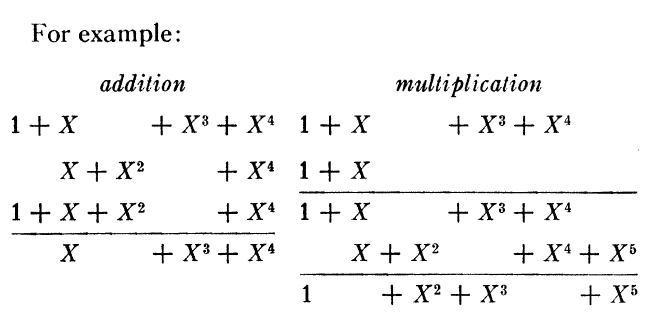
\includegraphics[scale=0.35]{imagenpp.png} 
In addition to the associative, distributive, and commutative properties of polynomials under this kind of algebra, we have, as in ordinary algebra, unique factorization; that is, every, polynomial can be factored into prime or irreducible factors in only one way. See[1]
To determine the checksum of a number, the remainder of the division using mod 2 is used, because only the remainder is needed the division algorithm is simplified and does not keep count of the quotient. The checksum is added to the message and this is sent to the receiver, if the receiver receives data that is not divisible by the divisor used on the algorithm, there was an error in the transaction. 
\section{Experiments}
For the experiments of the CRC we got a version that were made by Nicco Kunzmann from the Massachusetts Institute of Technology where were taken 7 entries of different size to see the difference between the results.
The entries are of 27, 100, 500, 1000, 10000, 100000 and 1000000 bytes, the intervals are to get a higher difference between their results.
The distinct parameters used for the runs are “lorem ipsum” texts, which are pseudo-random character arrays generated using an online tool.
A total of 30 experiments took place, each with different inputs. These experiments threw fairly similar results, therefore in the next three charts summarize the results. \\
\textbf{Experiment 1}\\
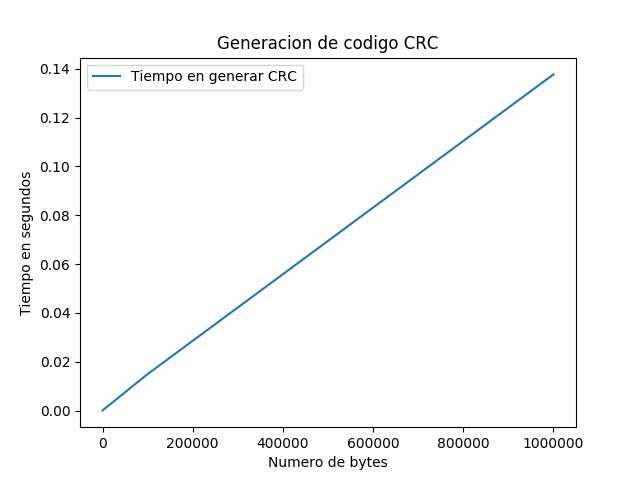
\includegraphics[scale=0.4]{figura1.png}
\begin{tabular}{ l | c | r }
  \hline			
  \#Bytes & Time & Output \\ \hline
  27 & $6.98*10^{-5}$ & 0xED \\
  100 & $1.07*10^{-4}$ & 0x9F \\
  1000 & $2.35*10^{-4}$ & 0xA4 \\
  10000 & $1.72*10^{-3}$ & 0x03 \\
  100000 & $1.42*10^{-2}$ & 0x1E \\
  1000000 & $1.28*10^{-1}$ & 0x84 \\
  \hline  
\end{tabular}\\
\textbf{Experiment 2}\\
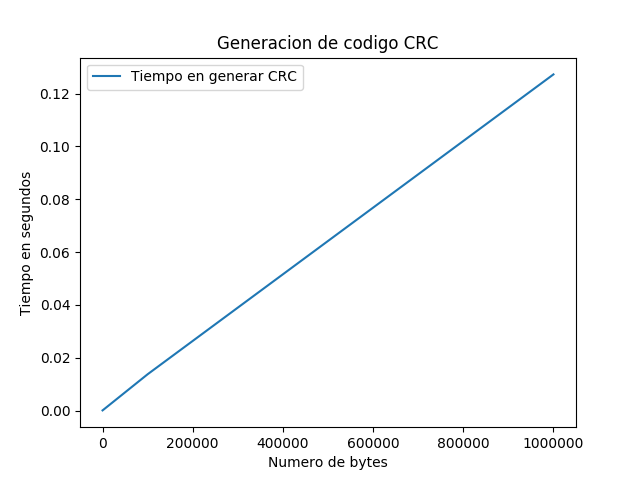
\includegraphics[scale=0.4]{figura2.png} \\
\begin{tabular}{ l | c | r }
  \hline			
  \#Bytes & Time & Output \\ \hline
  27 & $4.57*10^{-5}$ & 0xED \\
  100 & $5.55*10^{-5}$ & 0x9F \\
  1000 & $1.78*10^{-4}$ & 0xA4 \\
  10000 & $1.41*10^{-3}$ & 0x03 \\
  100000 & $1.415*10^{-2}$ & 0x1E \\
  1000000 & $1.27*10^{-1}$ & 0x84 \\
  \hline  
\end{tabular}\\
\textbf{Experiment 3}\\
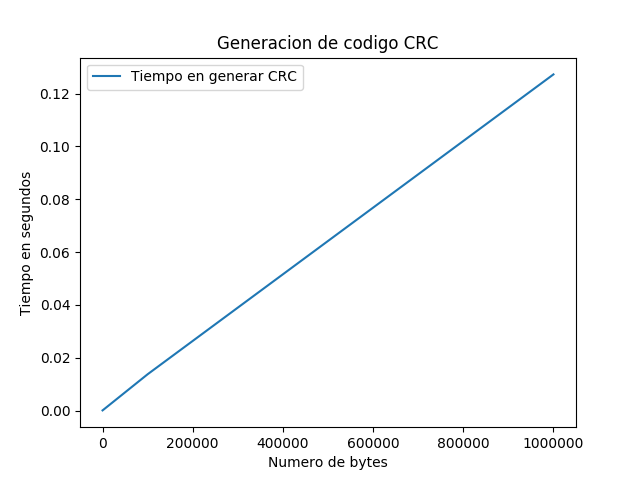
\includegraphics[scale=0.4]{figura2.png}\\
\begin{tabular}{ l | c | r }
  \hline			
  \#Bytes & Time & Output \\ \hline
  27 & $4.81*10^{-5}$ & 0xED \\
  100 & $5.55*10^{-5}$ & 0x9F \\
  1000 & $1.76*10^{-4}$ & 0xA4 \\
  10000 & $1.38*10^{-3}$ & 0x03 \\
  100000 & $1.397*10^{-2}$ & 0x1E \\
  1000000 & $1.263*10^{-1}$ & 0x84 \\
  \hline  
\end{tabular}\\
\section{Analysis of results}
The time spent by the CRC algorithm was generally constant, at large scale the algorithm's behavior did match the expected linear output. Therefore it is possible for people to calculate how many time will take to process $n$ bytes because of the constant polynomial average result.
As it is visible in the graphics, the function effectively came out to be similar in growth to a linear function, with some irregularities that can be discarded once the inputs are large enough. This was possible to observe thanks to to the distances in size of the byte-arrays that were given in as parameters.

\section{Conclusions}
In synthesis, the CRC is a variant algorithm and also trusty to find unwanted elements in the data transfer, where the variation comes from distinct polynomials that can be used in different ways or entries to get the result we want. And we got the final conclusion that the general polynomial method can work correctly and in similar way for all the entries letting the researchers to calculate how many time could an entry take to be processed.

\section{References}
[1]   W.W. Peterson “Cyclic Codes for Error Detection”, p.229, 1961 
[2] “Calculating the Hamming Code”, [Online] Available: 
\href{http://users.cis.fiu.edu/~downeyt/cop3402/hamming.html}{http://users.cis.fiu.edu/~downeyt/cop3402/hamming.html}. 

[3] “A Painless Guide to CRC Error Detection Algorithms”, [Online] Available:
\href{http://www.zlib.net/crc_v3.txt}{http://www.zlib.net/crc\_v3.txt}\\
\href{http://scanftree.com/programs/c/c-program-to-implement-crc-cyclic-redundancy-code/}{http://scanftree.com/programs/c/c-program-to-implement-crc-cyclic-redundancy-code/}\\
\href{http://vision.lakeheadu.ca/engi2453/lab/experiment1.html}{http://vision.lakeheadu.ca/engi2453/lab/experiment1.html}\\
\href{https://www.eee.hku.hk/~sdma/elec7073/Part2-2-Cyclic\%20redundancy\%20check\%20(CRC).pdf}{https://www.eee.hku.hk/~sdma/elec7073/Part2-2-Cyclic\%20redundancy\%20check\%20(CRC).pdf}\\
\href{http://vision.lakeheadu.ca/engi2453/lab/experiment1.html}{http://vision.lakeheadu.ca/engi2453/lab/experiment1.html}\\
\href{https://www.eee.hku.hk/~sdma/elec7073/Part2-2-Cyclic\%20redundancy\%20check\%20(CRC).pdf}{https://www.eee.hku.hk/~sdma/elec7073/Part2-2-Cyclic\%20redundancy\%20check\%20(CRC).pdf}\\
\href{www.lipsum.com}{www.lipsum.com}.\\
\href{https://pycrc.org/}{https://pycrc.org/}.


\end{document}